\section{Auswertung}

\subsection{Lichtgeschwindigkeitsmessung}

In den Abbildungen \ref{fig:x-f-remo} und \ref{fig:x-f-alex} sind die von Remo
Suter  und  Alex  Murray gemessene  Distanzenverschiebungen  in  Funktion  der
Drehfrequenz $f$ aufgezeichnet.

\begin{figure}[H]
    \center
    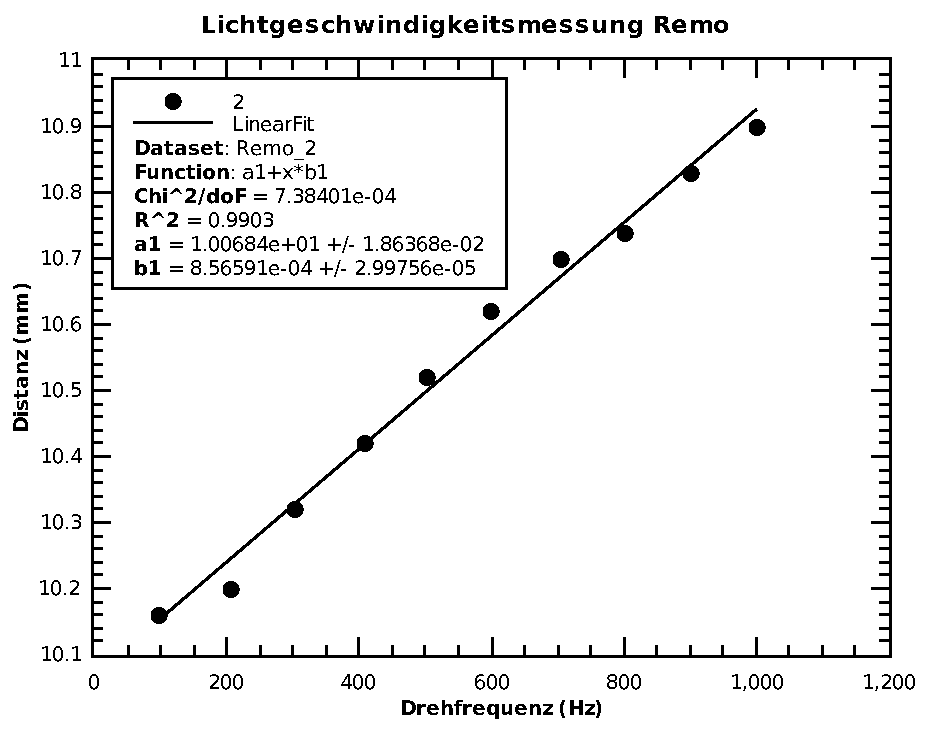
\includegraphics[width=.65\textwidth]{images/x-f-remo.pdf}
    \caption{Lineare Regression zur Berechnung des Faktors $b_1$, Messdaten von Remo Suter}
    \label{fig:x-f-remo}
\end{figure}

\begin{figure}[H]
    \center
    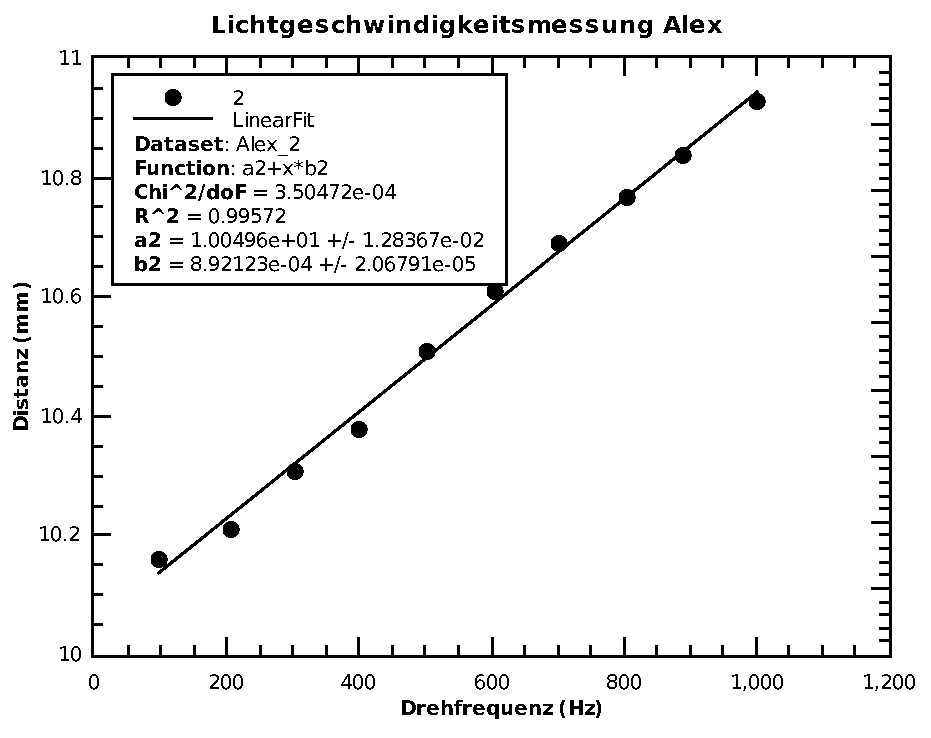
\includegraphics[width=.65\textwidth]{images/x-f-alex.pdf}
    \caption{Lineare Regression zur Berechnung des Faktors $b_1$, Messdaten von Alex Murray}
    \label{fig:x-f-alex}
\end{figure}

Die Punkte wurden nach der Formel \ref{eq:lichtgeschwindigkeit} gefittet und damit ergeben sich  die zwei  Faktoren:
\begin{align*}
    b_{1,Remo} &= \overline{b_{1,Remo}} \pm s_{\overline{b_{1,Remo}}} = (856.59 \pm 29.96)\cdot 10^{-9} \\
    b_{1,Alex} &= \overline{b_{1,Alex}} \pm s_{\overline{b_{1,Alex}}} = (892.12 \pm 20.68)\cdot 10^{-9}
\end{align*}


\subsection{Kalibrationsmessung}

In   den  abbildungen  \ref{fig:z-x-remo}  und  \ref{fig:z-x-alex}  sind   die
Kalibrationsmessungen von Remo Suter Alex  Murrayaufgef\"uhrt. Beide haben die
gleiche Messung unabh\"angig von einander durchgef\"uhrt.

\begin{figure}[H]
    \center
    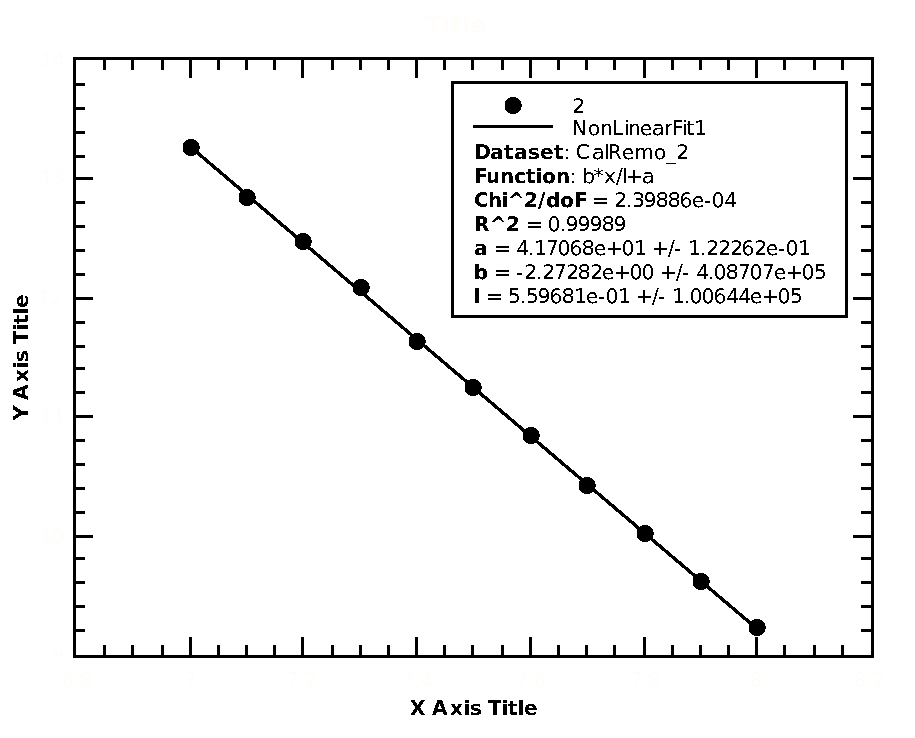
\includegraphics[width=.65\textwidth]{images/z-x-remo.pdf}
    \caption{Lineare Regression zur Berechnung des Faktors $b_2$ anhand der Kalibrationsmessung, Messdaten von Remo Suter}
    \label{fig:z-x-remo}
\end{figure}

\begin{figure}[H]
    \center
    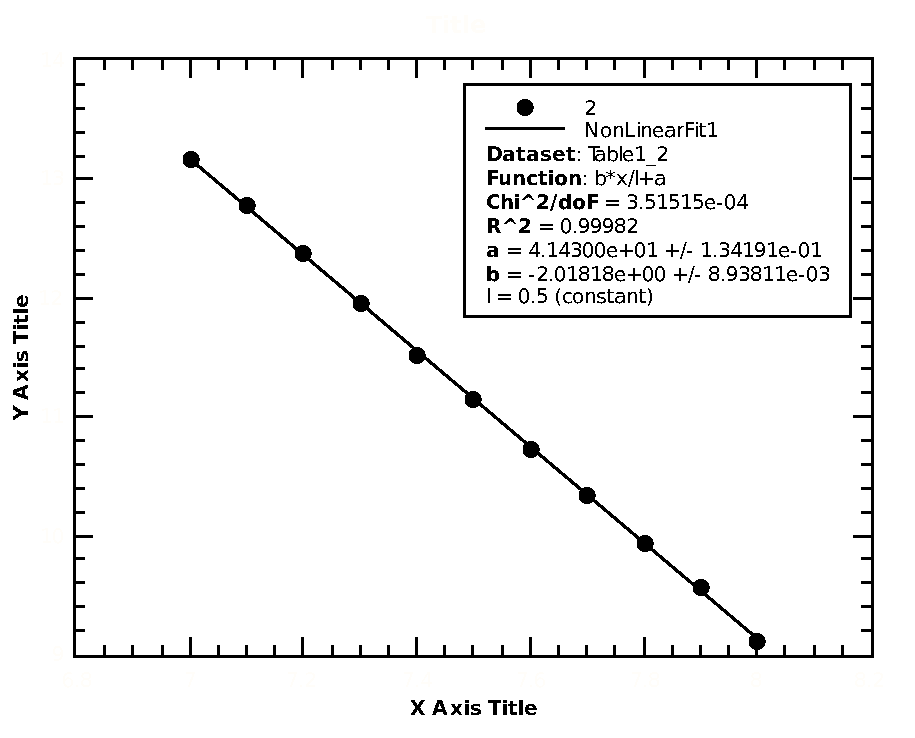
\includegraphics[width=.65\textwidth]{images/z-x-alex.pdf}
    \caption{Lineare Regression zur Berechnung des Faktors $b_2$ anhand der Kalibrationsmessung, Messdaten von Alex Murray}
    \label{fig:z-x-alex}
\end{figure}

Die Punkte wurden nach  der  Formel  \ref{eq:kalibration-a} gefittet und somit
ergeben sich der Faktoren

\begin{align*}
    b_{2,Remo} &= \overline{b_{2,Remo}} \pm s_{\overline{b_{2,Remo}}} = -(2030.5 \pm 7.0)\cdot 10^{-3} \\
    b_{2,Alex} &= \overline{b_{2,Alex}} \pm s_{\overline{b_{2,Alex}}} = -(2018.2 \pm 8.9)\cdot 10^{-3}
\end{align*}

